{
    \color{red}
    \begin{enumerate}
        \item Biological background
        \begin{enumerate}
            \item residue identity prediction
            \item atomic environments 
            \item SMILES representation?
        \end{enumerate}
        \item Machine learning background
        \begin{enumerate}
            \item neural networks
            \item graph neural networks
            \item equivariant graph neural networks
            \item representing residues as graphs
        \end{enumerate}
    \end{enumerate}
}

\section{Biological background}
\subsection{Proteins}
Amino acids are the building blocks of proteins and play a fundamental role in various biological processes. These small organic molecules are essential for life, and their unique properties allow them to form complex and diverse structures within the body. 
All amino acids follow the same underlying pattern and consist of a central carbon atom (C), an \textit{amino} group ($\text{NH}_3$), a \textit{carboxyl} group (COOH), and a variable side-chain, as we can see in Figure \ref{fig:amino-acid}.
Chains of amino acids are formed through a chemical reaction that creates a \textit{peptide bond}, as shown in Figure \ref{fig:residue}. The portions left of the original amino acids are called \textit{residues}. Note that there are 20 naturally occuring amino acids.
\begin{figure}
    \centering
    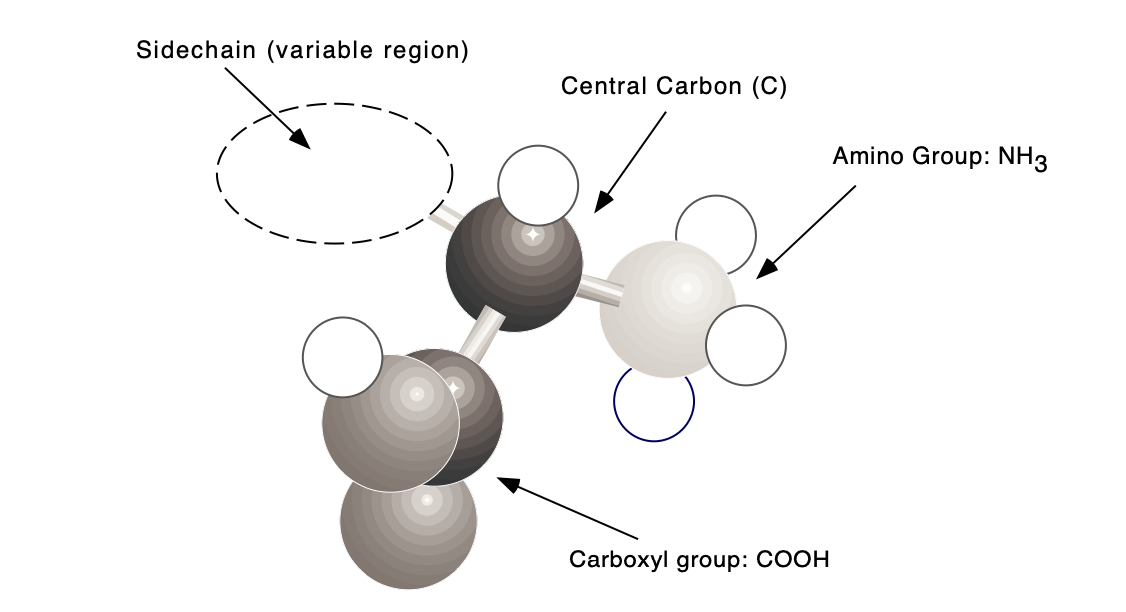
\includegraphics[scale=0.5]{figures/amino-acid.png}
    \caption{The basic chemical structure of an amino acid. Carbon atoms are black, Oxygen is dark grey, Nitrogen light grey, and hydrogen white. Image taken from \cite{hunter1993molecular}.}
    \label{fig:amino-acid}
\end{figure}

\begin{figure}
    \centering
    \begin{tikzpicture}
    \node (acidone) {\chemfig[atom sep=2em]{N(-[3]H)(-[5]H)-C(-[2]H)(-[6]R_1)-C(-[1]{\color{blue}OH})(=[7]O)}};
    \node[right of=acidone, xshift=3cm] (acidtwo) {\chemfig[atom sep=2em]{N(-[3]H)(-[5]{\color{blue}H})-C(-[2]H)(-[6]R_2)-C(-[1]OH)(=[7]O)}};
    \draw[->,thick] ($(acidone.east)!0.5!(acidtwo.west)$) ++(0, -1.2cm) -- ++(0,-0.8cm) node[right] {};
    \node[below of=acidone, xshift=2cm, yshift=-2.4cm] (residue) 
        {\chemfig[atom sep=2em]{N(-[3]H)(-[5]H)-C(-[2]H)(-[6]R_1)-C(=[7]O)-[1,,,,blue]N(-[3]H)-C(-[2]H)(-[6]R_2)-C(=[7]O)(-[1]OH)}};
    
    \node[below of=residue, yshift=-0.7cm, xshift=-1.5cm] (res1) {\textit{residue 1}};
    \node[below of=residue, yshift=-0.7cm, xshift=1.5cm] (res1) {\textit{residue 2}};
    \end{tikzpicture}
    \caption{Two amino-acids are chained together through a peptide bond. The chemical reaction releases a water molecule ($\text{H}_2\text{O}$) in the process.}
    \label{fig:residue}
\end{figure}
Proteins are one of the most important macromolecules found in living organisms and they are involved in a vast array of biological processes. 
These large, complex molecules are composed of long chains of amino acids that are folded into shapes.
Proteins play a variety of roles in the body, including catalysing chemical reactions, transporting molecules, providing structural support, and regulating gene expression. 
The diversity of protein structures and functions is vast, with some proteins consisting of just a few amino acids, while others contain thousands. 
The unique sequence of amino acids in each protein determines its three-dimensional structure and, more importantly, its \textit{specific function}. 
Understanding the structure and function of proteins is essential for advancing our knowledge of cellular processes and for developing treatments for a range of diseases caused by protein dysfunction.
\subsection{Residue identity prediction}
Residue identity prediction (RES) is a computational task in bioinformatics that involves predicting the amino acid residue at a particular position within a protein sequence. 
The accurate prediction of residue identity is an important problem in bioinformatics because it can provide insights into protein function, structure, and evolution. 
Knowing the identity of residues within a protein sequence can help to identify important functional sites and motifs, which can provide clues about the protein's function and interactions with other molecules. 

Residue identity prediction is also important for \textit{protein engineering}, as it can help researchers design proteins with specific functions.
Machine learning approaches to RES have already been used to engineer plastic decomposing enzymes for higher thermal stability \cite{Lu2022}.

\paragraph{The ATOM3D dataset.} One important benchmark dataset for RES is ATOM3D \cite{atom-3d}.
The ATOM3D collection is a compilation of datasets that contain the 3D structure of biomolecules, including nucleic acids, small molecules, and proteins. 
These datasets have been tailored to function as a benchmark for machine learning techniques that train on the 3D molecular structure of molecules in order to solve tasks such as molecular function prediction, ligand binding affinity, or protein-protein interactions.

\paragraph{The PDB format.} ATOM3D datasets have a standardised format, in which each sample is a \texttt{.pdb} file. The \texttt{.pdb} format is a format provided by the \textbf{Protein Data Bank} (PDB), a database of 3D structural data of various biological molecules. Figure \ref{pdb} shows an example of a molecule from the PDB.
\begin{figure}
    \centering
    \subfigure[The 1KDA molecule. The orange structure represents one amino acid residue.]{
        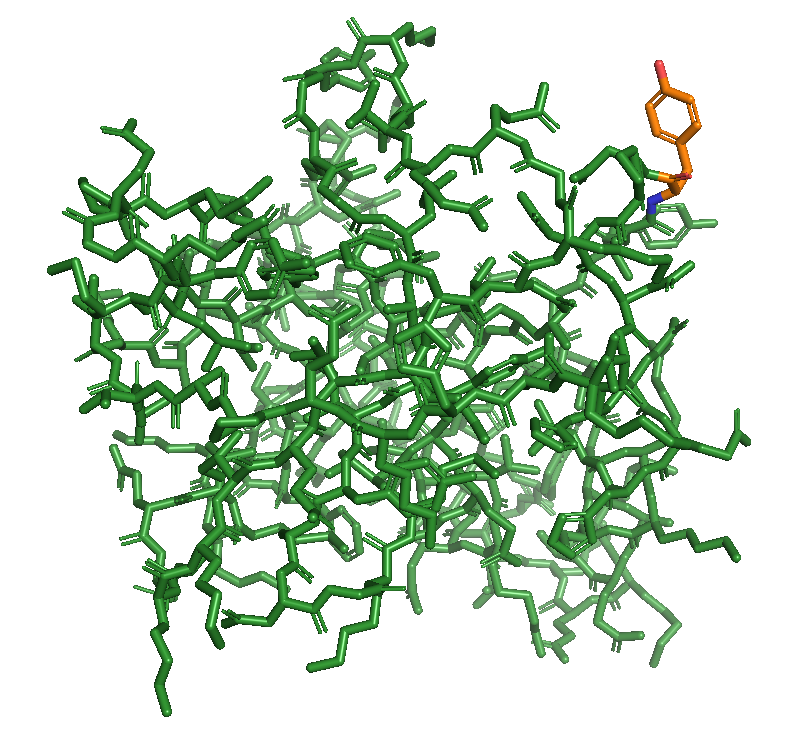
\includegraphics[scale=0.2]{figures/1kda_example.png}
    }
    \hspace{0.3in}
    \subfigure[A close-up of the atomic environment around the orage amino-acid.]{
        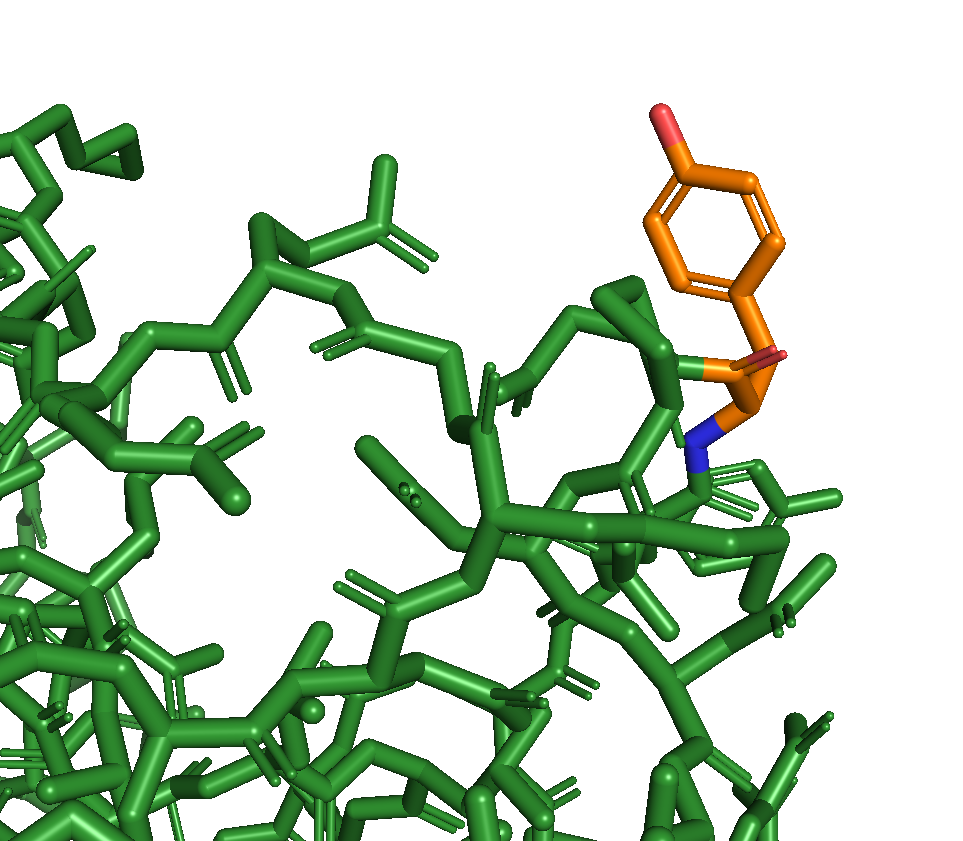
\includegraphics[scale=0.2]{figures/1kda_closeup.png}
    }
    
    \caption{Example of a PDB molecule.}
    \label{pdb}
\end{figure}
\section{Machine learning background}
First proposed by \citet{rosenblatt1958}, neural networks are a type of machine learning model that is inspired by the structure and function of the human brain. 
They are used for various tasks, such as image and speech recognition, natural language processing, and biomolecular prediction among others.

At a high level, neural networks consist of interconnected nodes or neurons organised into layers. Each neuron receives input data, applies a mathematical operation to it, and produces an output. These operations are typically weighted sums followed by activation functions that introduce non-linearity into the model. 
The outputs from one layer of neurons serve as inputs to the next layer, forming a hierarchical structure. The resulting predictions made by the model are then scored using a \textit{loss function}.

The training process in neural networks involves two steps. First, the derivative of the loss function with respect to each weight is computed, using the \textit{backpropagation algorithm} \citep{backpropagation1}. This provides the gradient information needed for the next step. The second stage is the weight update, typically done using a gradient descent technique. 

\subsection{Graph Neural Networks}
{\color{blue}Maybe flesh this out later.}

\textbf{Graph neural networks} (GNNs) are a type of neural network that operate on graphs and are able to capture structural information in the data by leveraging the existent relationships between entities. 
All GNNs use some form of \textit{neural message passing}, where vector messages are exchanged between nodes and updated using a neural network \citep{gilmer2017neural}.

Formally, for a given graph $\mathcal{G} = (\mathcal{V}, \mathcal{E})$, at message passing iteration $k$, a hidden embedding $\textbf{h}_u^{(k)} \in \mathbb{R}^{F_k}$ corresponds to each node $u \in \mathcal{V}$. 
The framework first creates a \textit{message} $\mathbf{m}_{u,v}$ between a node $u$ and its neighbour $v$ by using a message function $\psi^{(k)}: \mathbb{R}^{F_k}\times\mathbb{R}^{F_k} \rightarrow \mathbb{R}^{F_{k}'}$:
\begin{equation}
    \mathbf{m}_{u, v} = \psi^{(k)}\Big(\textbf{h}_{u}^{(k)}, \textbf{h}_v^{(k)}\Big)
\end{equation}
These messages are then aggregated using operation $\oplus^{(k)}$; 
this operation is usually the sum or the average, but other versions exist as well. Note that in general function must be \textit{permutation invariant}, since the neighbours of a node $u$ do not have any intristic order.
Finally, the aggregated message is combined with the node's own embedding $\mathbf{h}_u^{(k)}$ using function $\phi^{(k)}:\mathbb{R}^{F_k} \times \mathbb{R}^{F_{k}'} \rightarrow \mathbb{R}^{F_{k+1}}$, also called the \textit{update} function, as seen in Equation \ref{message-passing}:
\begin{align}
    \textbf{h}_u^{(k+1)} &= \phi^{(k)}\Big(\textbf{h}_u^{(k)}, \oplus_{v\in \mathcal{N}(u)}^{(k)}\mathbf{m}_{u,v}\Big)
\label{message-passing}
\end{align}

A visual representation of the information flow can be seen in Figure \ref{message_passing_fig}.
\begin{figure}
    \centering
    \begin{tikzpicture}[scale=0.6]
        % Graph
        \node (x1) [circle, draw=black, fill=red!20] {$\mathbf{x}_1$};
        \node (x2) [circle, draw=black, thick, fill=blue!20, below of=x1, yshift=-2cm, xshift=-4cm] {$\mathbf{x}_2$};
        \node (x3) [circle, draw=black, fill=blue!20, below of=x1, yshift=-2cm, xshift=4cm] {$\mathbf{x}_3$};
        \node (x4) [circle, draw=black, fill=blue!20, below of=x1, yshift=-2.5cm, xshift=1cm] {$\mathbf{x}_4$};

        
        \draw (x1) -- (x2);
        \draw (x1) -- (x3);
        \draw (x1) -- (x4);

        % Messages
        \node (m12) [circle, fill=green!30, above=of x2.center, xshift=0.7cm, yshift=0.3cm] {$\mathbf{m}_{1,2}$};
        \node (m13) [circle, fill=green!30, above=of x3.center, xshift=-0.7cm, yshift=0.3cm] {$\mathbf{m}_{1,3}$};
        \node (m14) [circle, fill=green!30, above=of x4.center, xshift=-1.3cm] {$\mathbf{m}_{1,4}$};

        \draw [->, dashed, gray, line width=1pt] (x1) -- (m14);
        \draw [->, dashed, gray, line width=1pt] (x4) -- (m14);
        % \draw [->, line width=2.5pt] (up1) .. controls (-0.25, 0.6) .. (x1);
        \draw [->, dashed, gray, line width=1pt] (x2) -- (m12);
        \draw [->, dashed, gray, line width=1pt] (x1) -- (m12);

        \draw [->, dashed, gray, line width=1pt] (x3) -- (m13);
        \draw [->, dashed, gray, line width=1pt] (x1) -- (m13);

        \node (update1) [circle, fill=orange!20, above=of x1.center, yshift=1cm] {$\oplus$};
        % \draw [->, line width=1.5pt] (m12) .. controls (-3, 0.5) .. (update1);
        \path (m12) edge[->, line width=1.2pt, bend left=30] (update1);
        \path (m14) edge[->, line width=1.2pt, bend left=30] (update1);
        \path (m13) edge[->, line width=1.2pt, bend right=30] (update1);
        \path (x1) edge[->, dashed, gray, line width=1pt, bend right=45] (update1);

        \draw [->, double, double distance=1pt, line width=1pt] (update1) -- (x1);
        \draw (x2) -- (x4);

        % \draw [->, line width=2pt] (m13) -- (up1);
    \end{tikzpicture}
    \caption{Diagram of the information flow of Equation \ref{message-passing}. Node $\mathbf{x}_1$ has three neighbours coloured in blue. The messages between node $\mathbf{x}_1$ and each of its neighbours are aggregated using operator $\oplus$; the result is used to update the embeddings of $\mathbf{x}_1$. Note how in this diagram we are not interested in the edge between $\mathbf{x}_2$ and $\mathbf{x}_4$, since this is the update iteration for node 1.}
    \label{message_passing_fig}
\end{figure}
\subsection{Equivariant Graph Neural Networks}
\begin{figure}
\centering
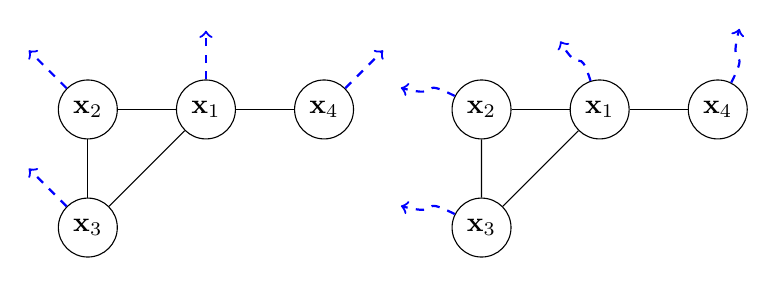
\begin{tikzpicture}
    \node[draw, circle] (x1) {$\mathbf{x}_1$};
    \node[draw, circle, left of=x1, xshift=-0.5cm] (x2) {$\mathbf{x}_2$};
    \node[draw, circle, below of=x2,  yshift=-0.5cm] (x3) {$\mathbf{x}_3$};
    \node[draw, circle, right of=x1,  xshift=0.5cm] (x4) {$\mathbf{x}_4$};
    
    \draw (x1) -- (x2);
    \draw (x1) -- (x4);
    \draw (x1) -- (x3);
    \draw (x2) -- (x3);

    \path[->] (x1) edge[out=90, in=270, looseness=2, blue, dashed, thick] ++(0,1);
    \path[->] (x2) edge[out=135, in=315, looseness=2, blue, dashed, thick] ++(-0.75,0.75);
    \path[->] (x4) edge[out=45, in=225, looseness=2, blue, dashed, thick] ++(0.75,0.75);
    \path[->] (x3) edge[out=135, in=315, looseness=2, blue, dashed, thick] ++(-0.75,0.75);

    \begin{scope}[rotate=30]
        \node[draw, circle, right of=x1, xshift=4cm] (x5) {$\mathbf{x}_1$};
        \node[draw, circle, left of=x5, xshift=-0.5cm] (x6) {$\mathbf{x}_2$};
        \node[draw, circle, below of=x6,  yshift=-0.5cm] (x7) {$\mathbf{x}_3$};
        \node[draw, circle, right of=x5,  xshift=0.5cm] (x8) {$\mathbf{x}_4$};
        
        \draw (x5) -- (x6);
        \draw (x5) -- (x8);
        \draw (x5) -- (x7);
        \draw (x6) -- (x7);
    
        \path[->] (x5) edge[out=90, in=270, looseness=2, blue, dashed, thick] ++(0,1);
        \path[->] (x6) edge[out=135, in=315, looseness=2, blue, dashed, thick] ++(-0.75,0.75);
        \path[->] (x8) edge[out=45, in=225, looseness=2, blue, dashed, thick] ++(0.75,0.75);
        \path[->] (x7) edge[out=135, in=315, looseness=2, blue, dashed, thick] ++(-0.75,0.75);
    \end{scope}
\end{tikzpicture}
\end{figure}

\subsection{Representing residues as graphs}
